\chapter{Results}

\section{Technological Systems}
Tables - no of buildings
tables  amount of land
\section{Natural Systems}
maps
\section{Social Systems}

\subsection{Summary Statistics of Survey Results}



\subsection{Interest Level in Sea Level Extremes}

\begin{figure}[h]
    \centering
    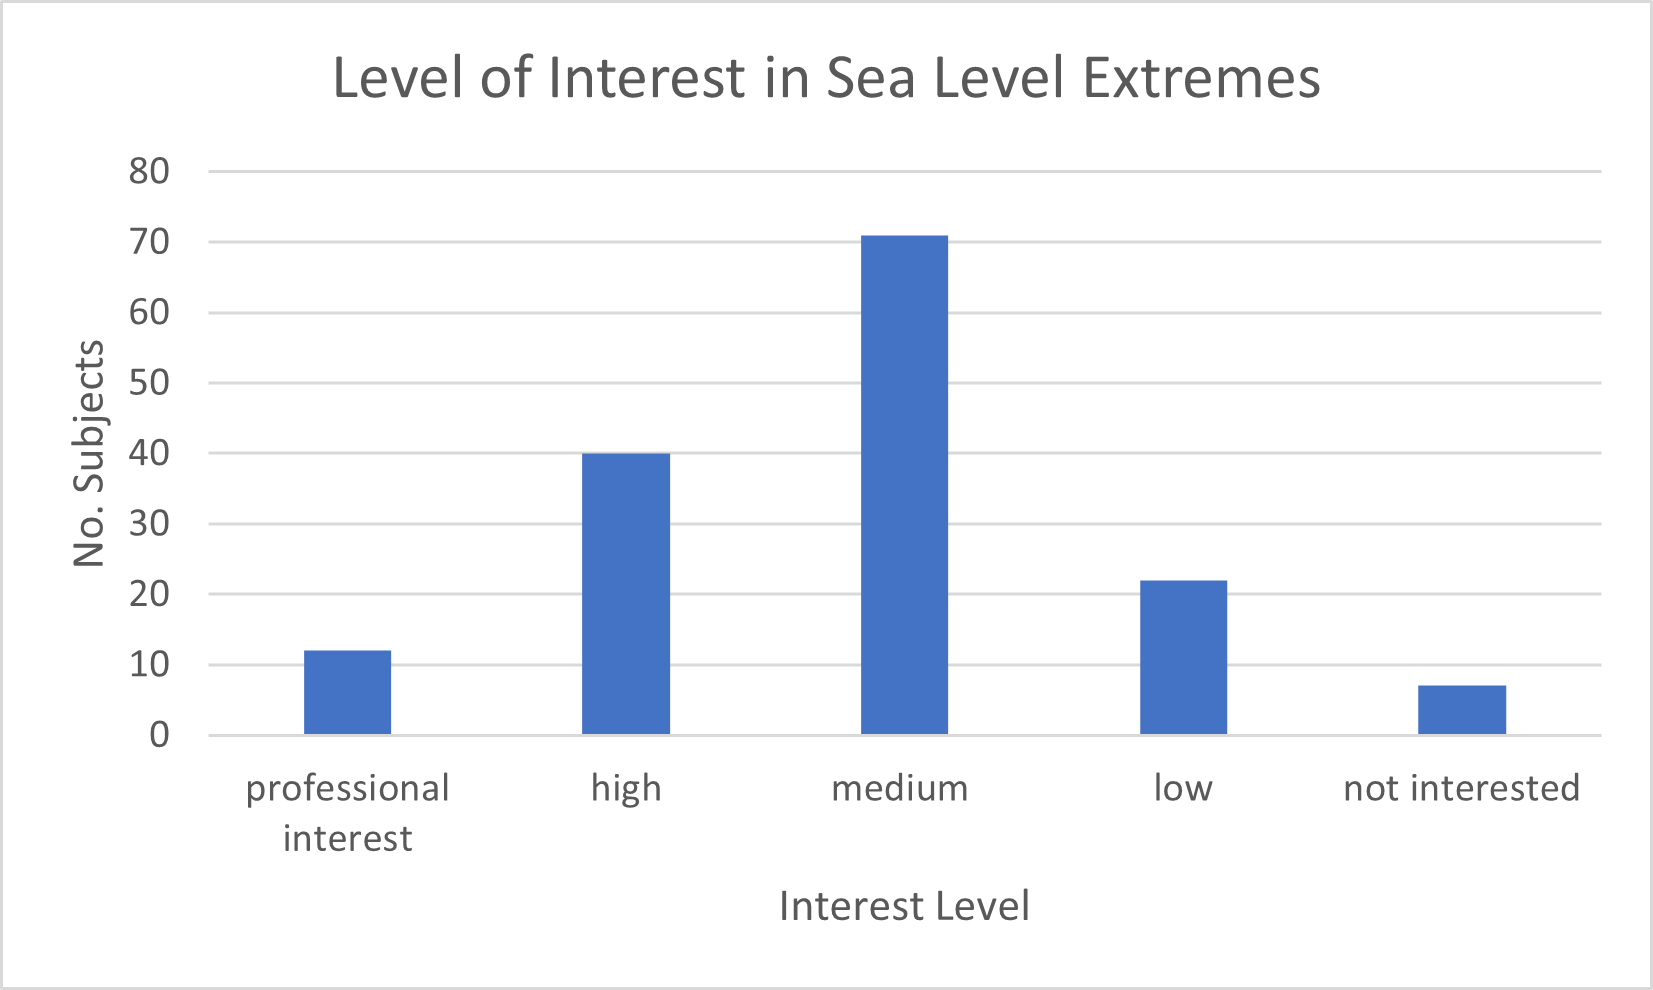
\includegraphics{fig_results/interest-level.png}
    \caption{Interest Level in Sea Level Extremes}
    \label{fig:my_label}
\end{figure}
\paragraph{}
words words words


\subsection{Memory of Sea Level Extremes}

\begin{figure}[h]
    \centering
    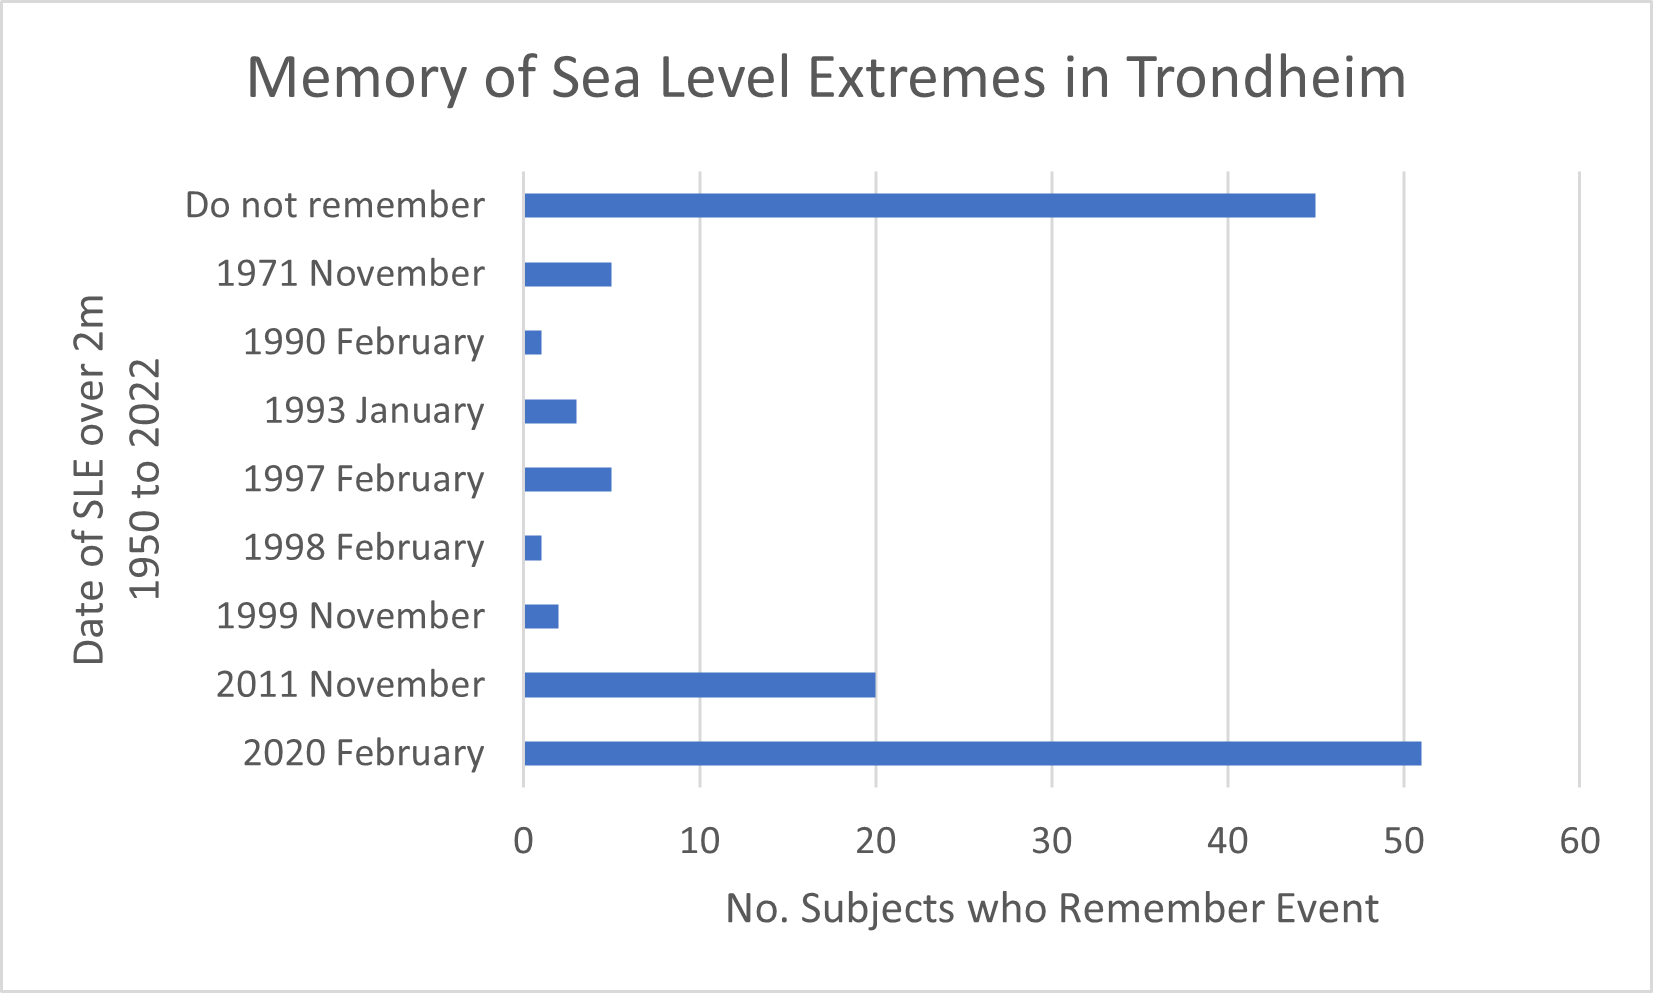
\includegraphics{fig_results/memory-sle.png}
    \caption{Memory of Sea Level Extremes}
    \label{fig:my_label}
\end{figure}
\paragraph{}
words words words
\subsection{Level of Interest in Sea Awareness}

\begin{figure}[h]
    \centering
    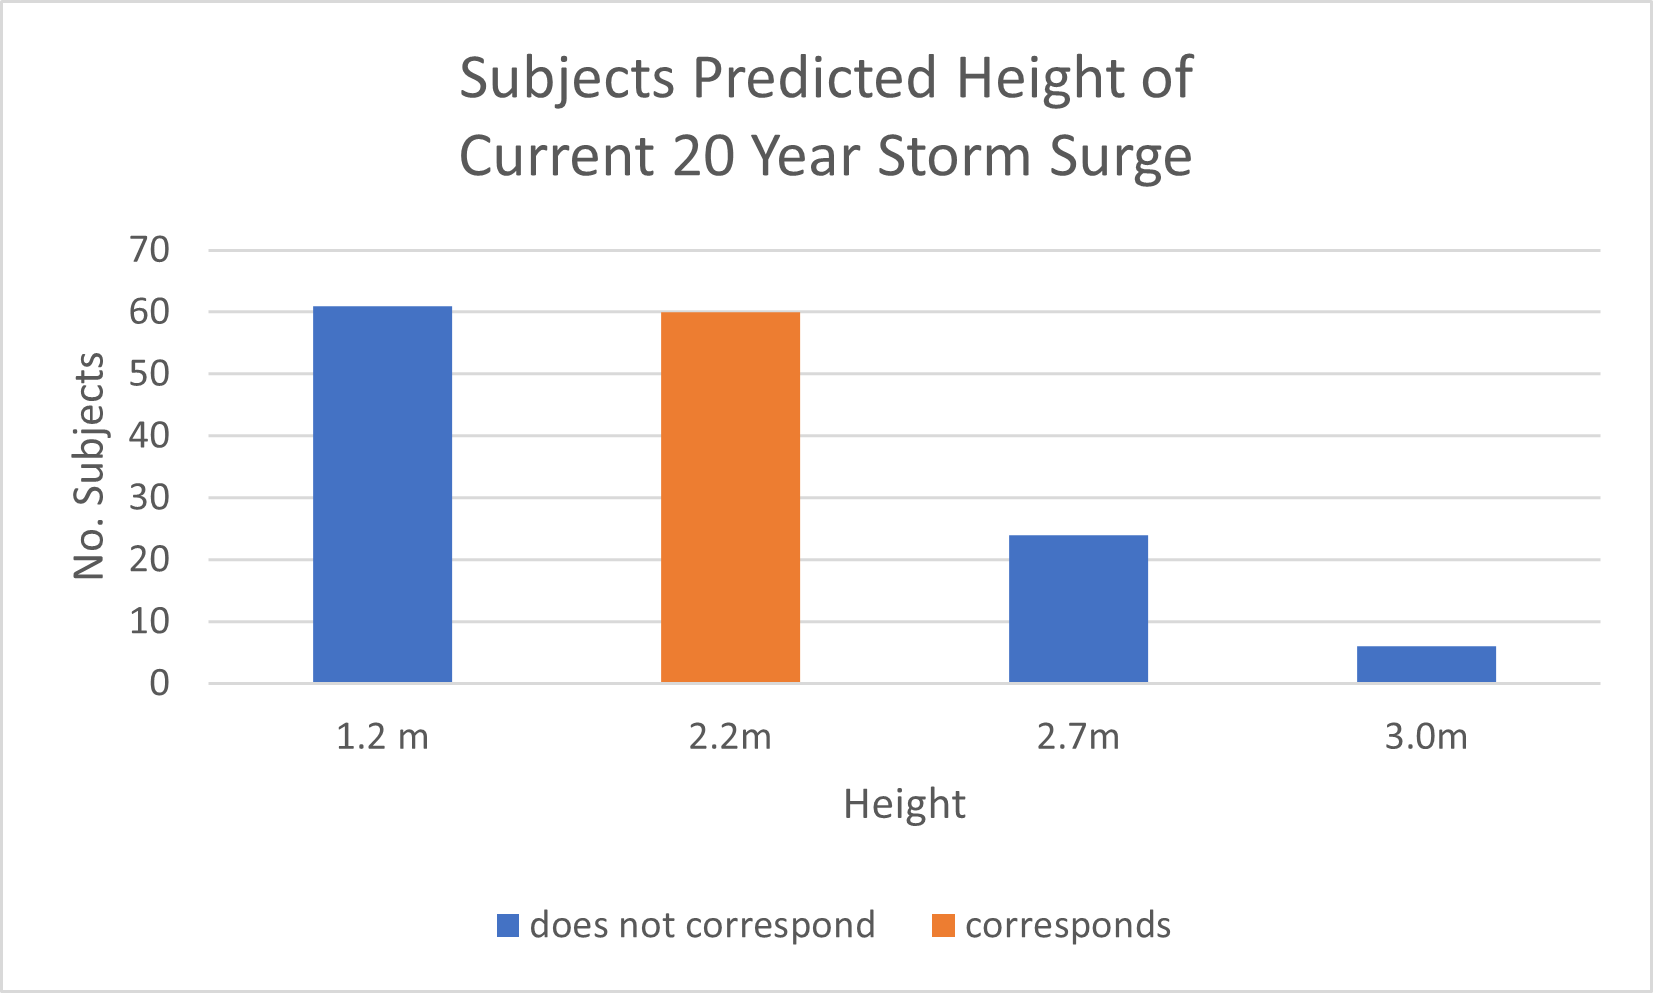
\includegraphics{fig_results/2022-20yrss-answer.png}
    \caption{Level of Interest in Sea Level Extremes}
    \label{fig:my_label}
\end{figure}
\paragraph{}
words word words

\subsection{Community Membership}

\begin{figure}
    \centering
    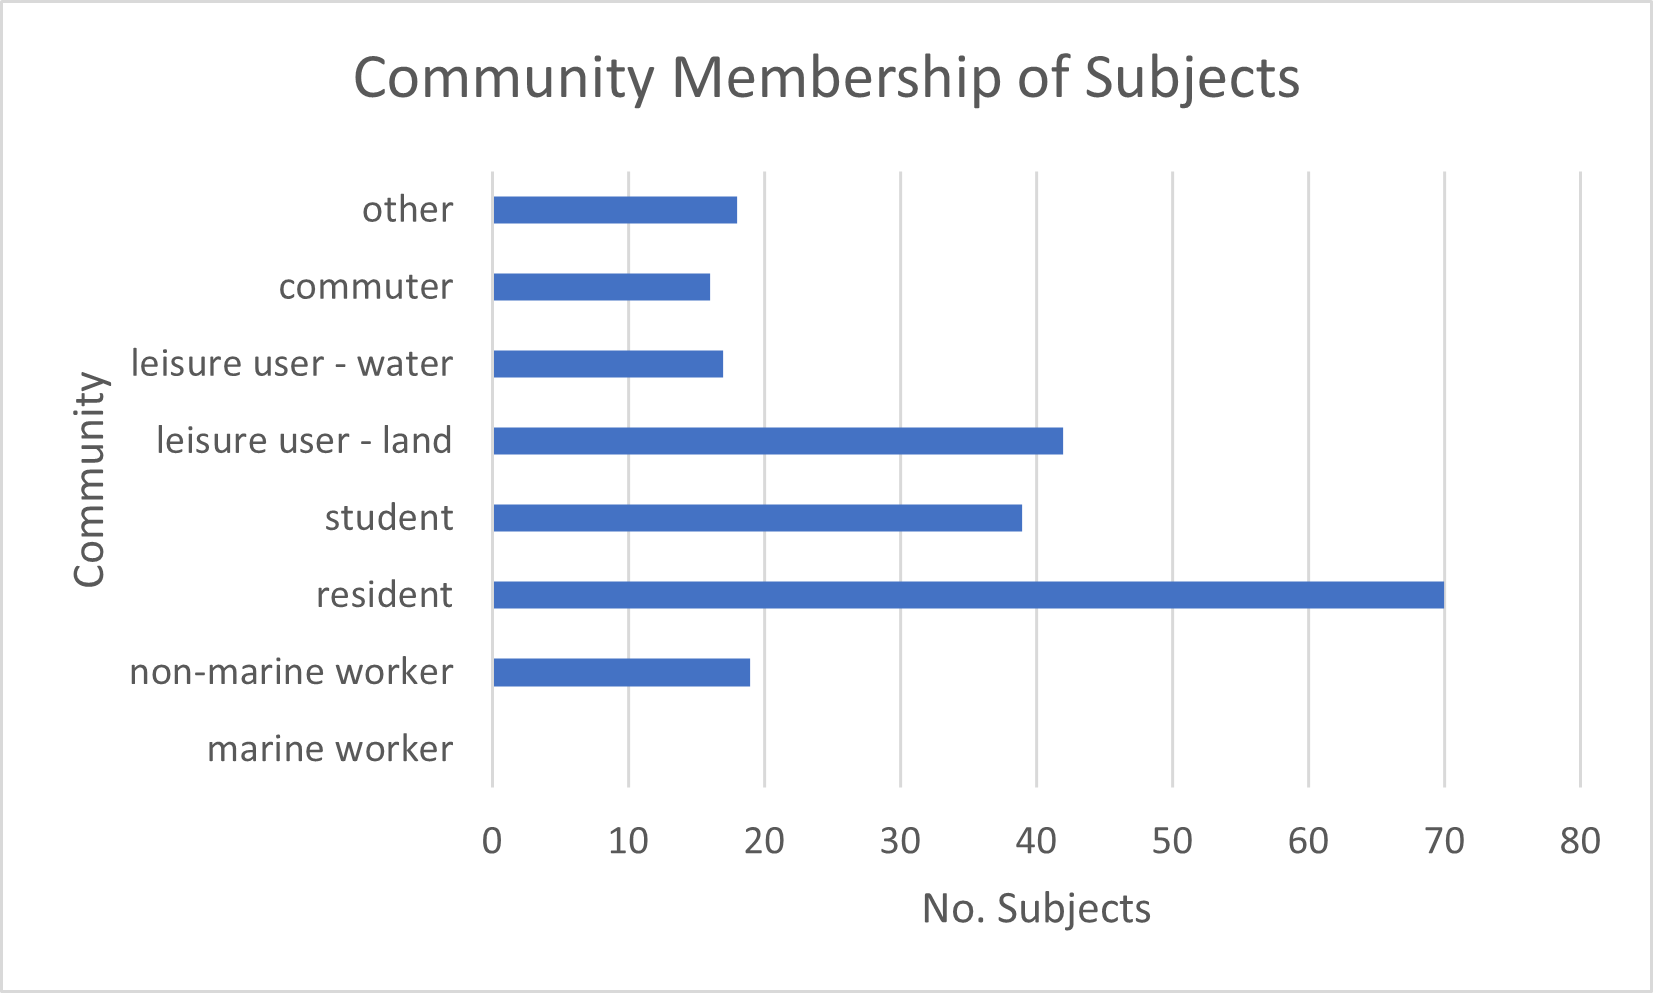
\includegraphics{fig_results/com-mem-horizontal.png}
    \caption{Membership of Communities}
    \label{fig:my_label}
\end{figure}
\paragraph{}
words words words 
\subsection{Access to Survey}

\begin{figure}[h]
    \centering
    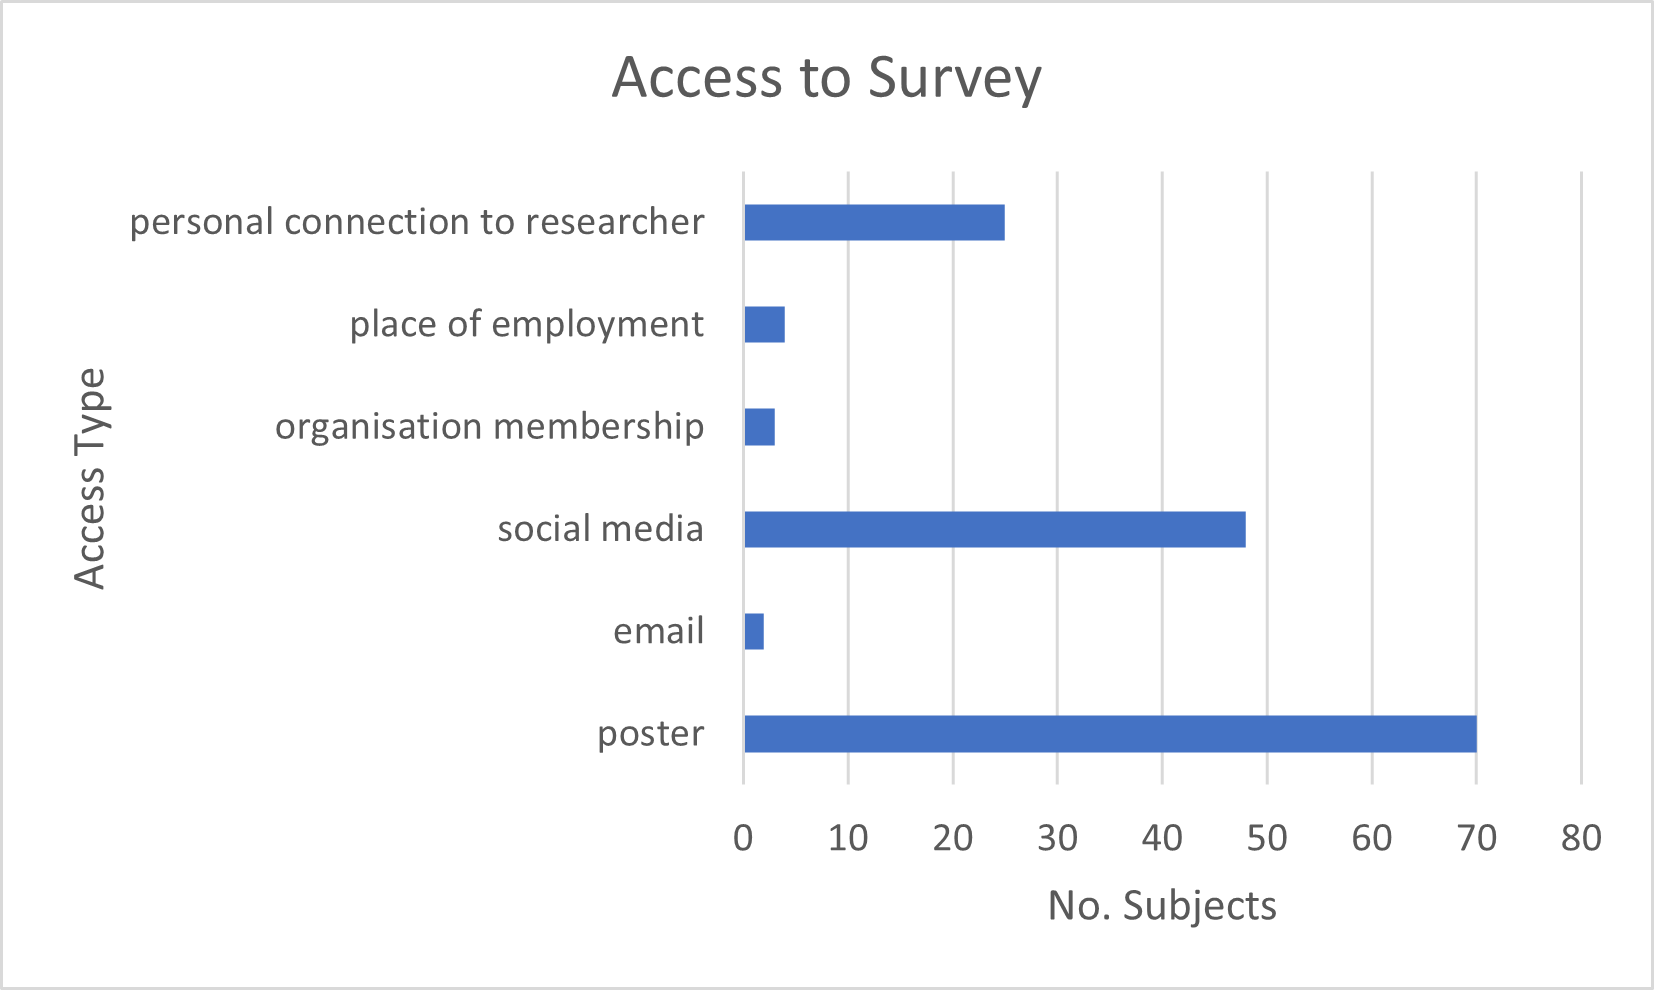
\includegraphics{fig_results/access_survey.png}
    \caption{Access to Survey}
    \label{fig:my_label}
\end{figure}
\paragraph{}
\subsection{Perceived Risks}

\begin{figure}[h]
    \centering
    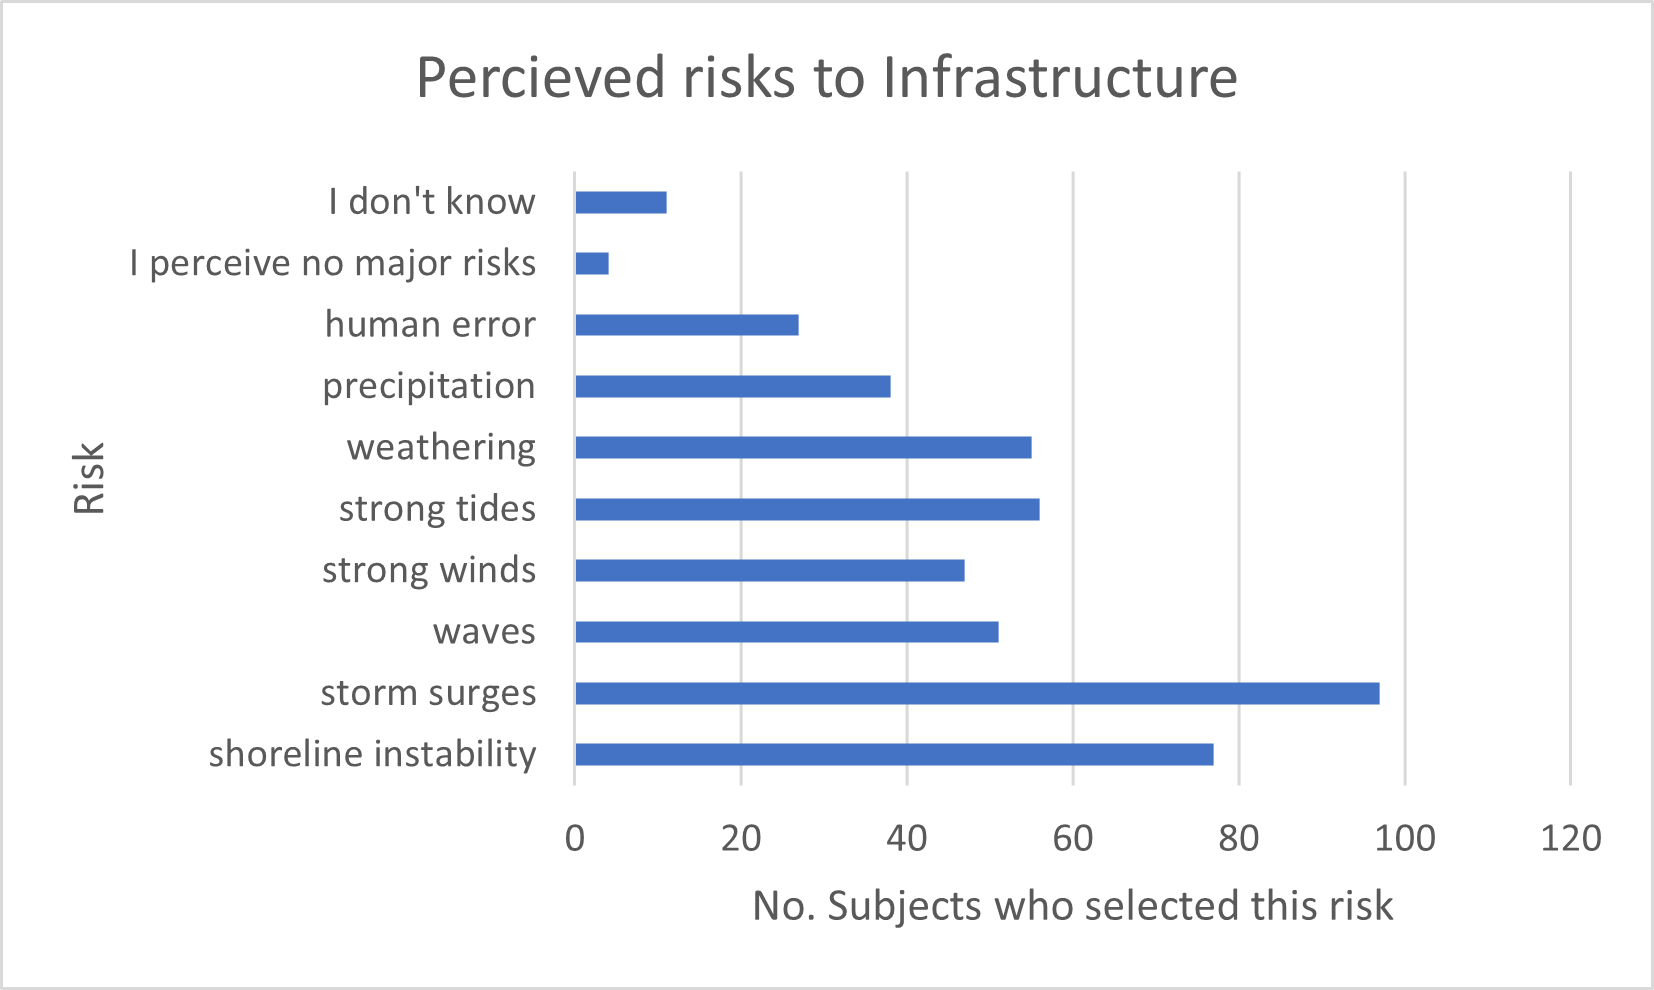
\includegraphics{fig_results/infrastructure-risks.png}
    \caption{Infrastructure Risks}
    \label{fig:my_label}
\end{figure}
\paragraph{}
words words words

\begin{figure}[h]
    \centering
    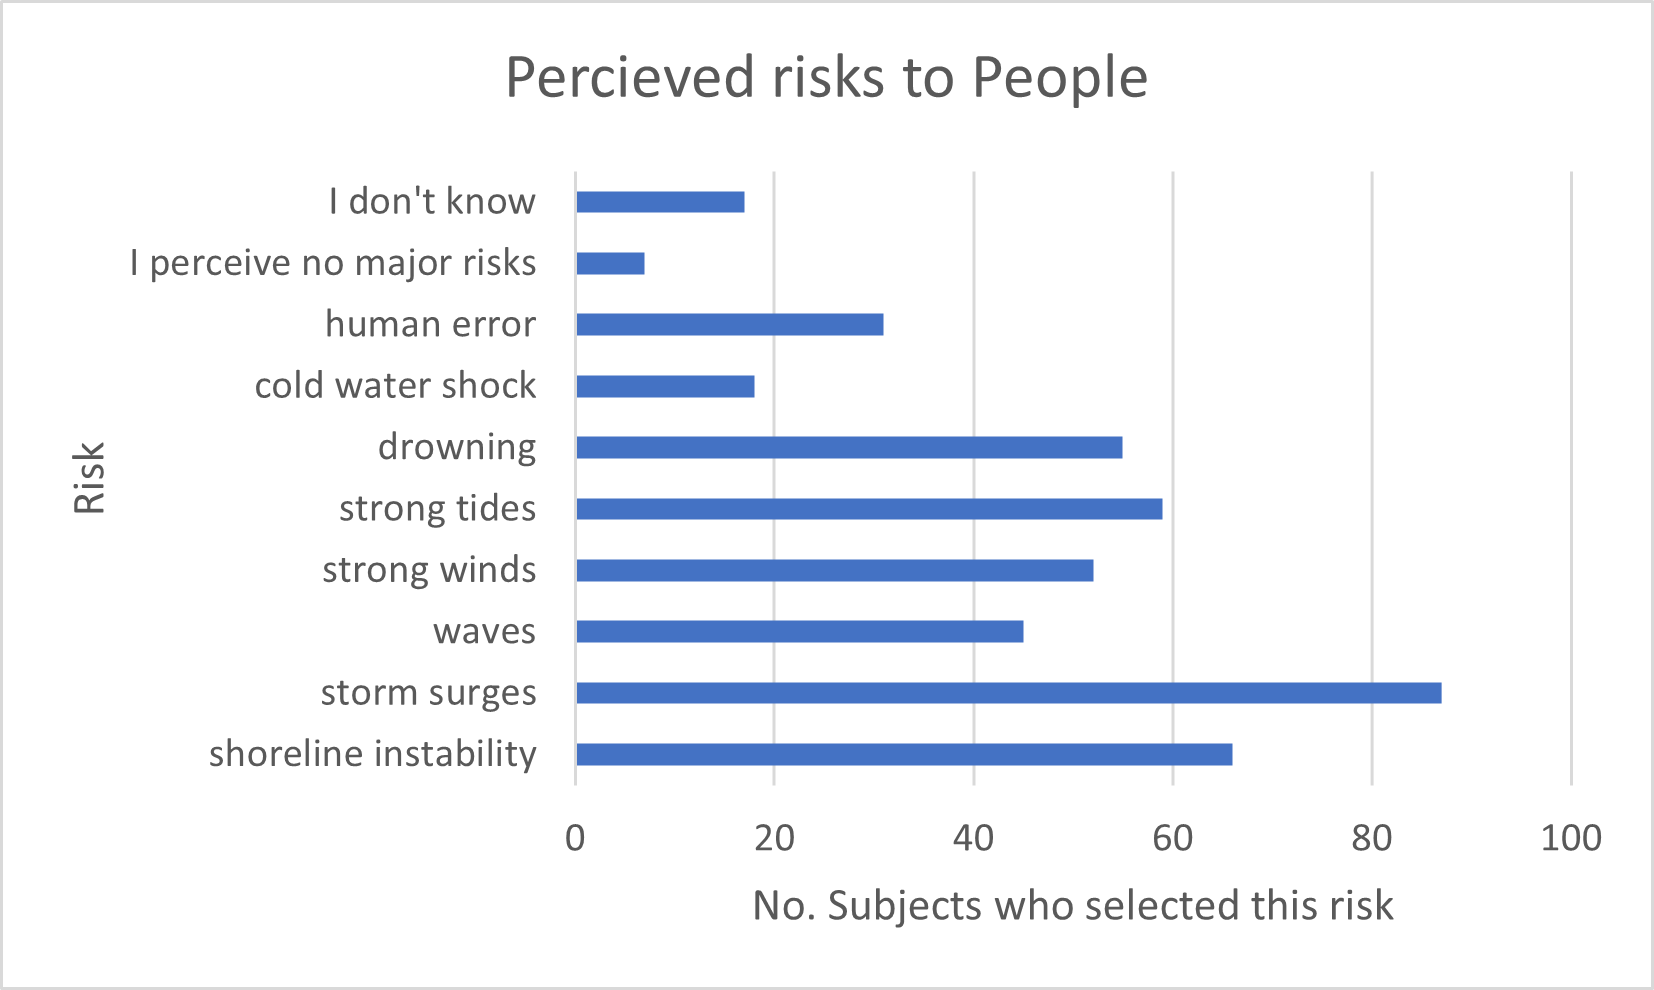
\includegraphics{fig_results/people-risks.png}
    \caption{People risks}
    \label{fig:my_label}
\end{figure}
\paragraph{}

\subsection{Awareness}

\begin{figure}[h]
    \centering
    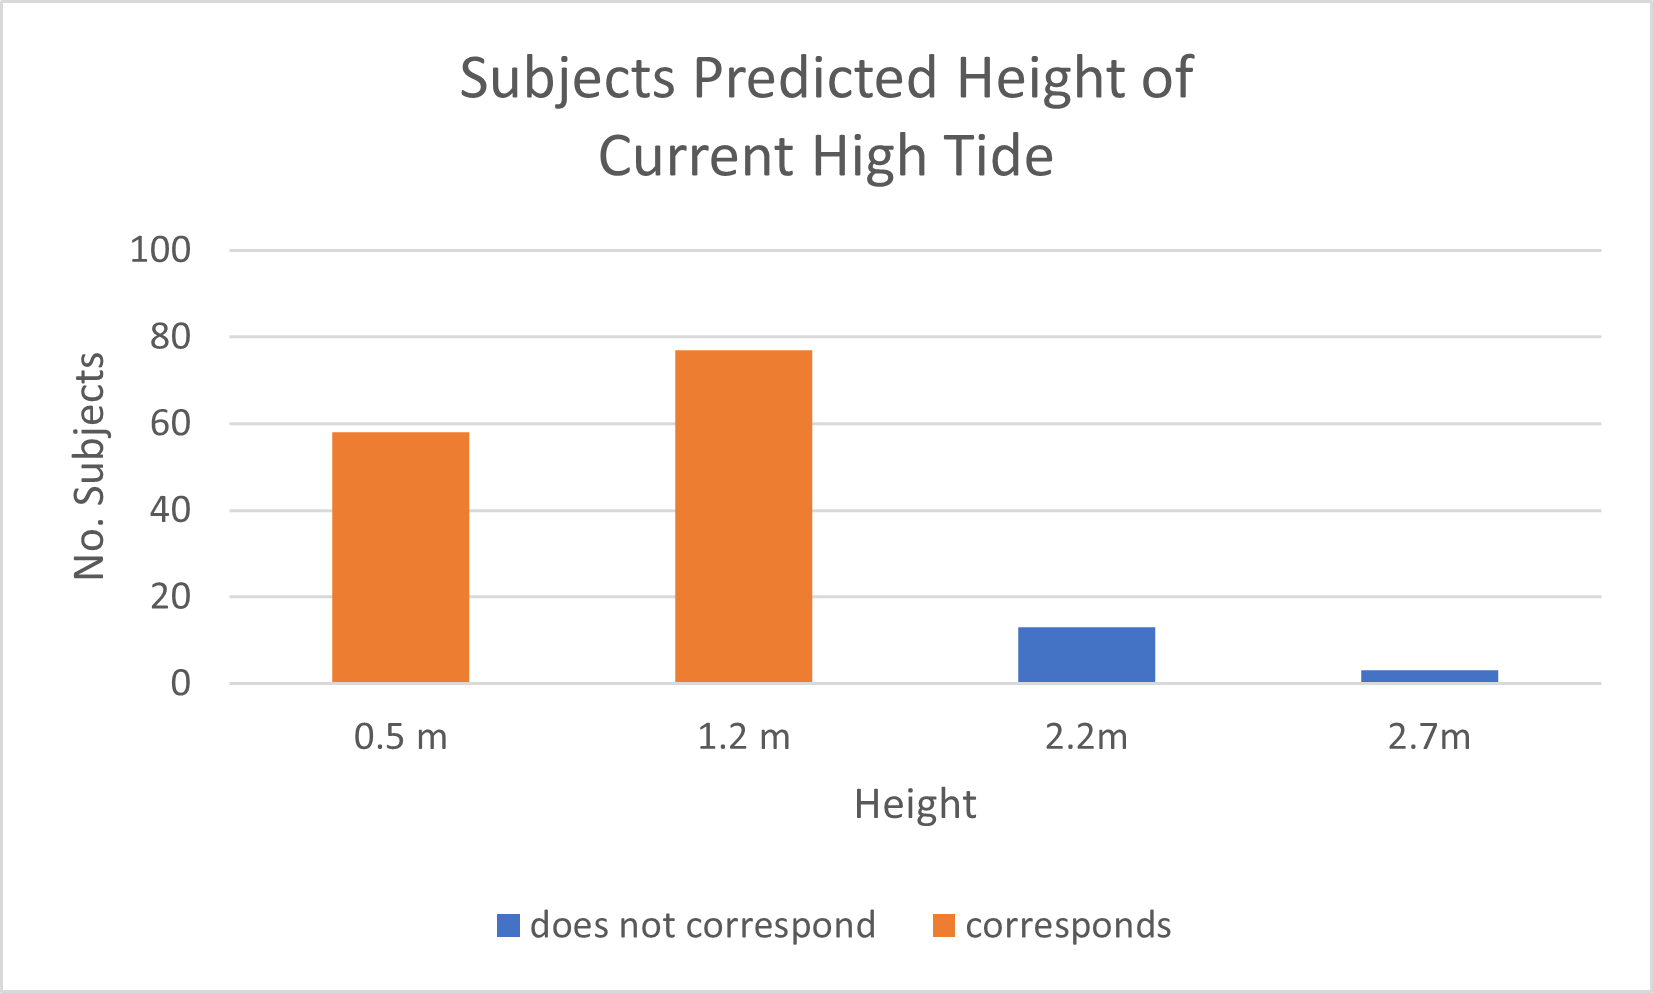
\includegraphics{fig_results/2022-hightide-answers.png}
    \caption{Subjects Predicted Height of Current High Tide. Height 0.5m is the neep high tide, Height 1.2m is the Spring High Tide. Th vast majority of subjects got an answer which corresponds with models of tides in Trondheim. Under 20 subjects responded with an answer which does not correspond with models of tides. 58 subjects chose 0.5m, 77 subjects chose 1.2m meaning that 135 out of 153 subjects, 88 percent chose what could be considered the correct answer for high tide. While only 13 subjects chose 2.2m and 3 subjects chose 2.7m}
    \label{fig:high-tide-answer}
\end{figure}
\paragraph{}
As can be seen in figure ** above the subjects displayed a high awareness of the tides in Trondheim. Under 20 subjects responded with an answer which does not reflect the models from \cite{kartverket_se_2021}. Over 88 percent of subjects chose a value which matches with models by \cite{kartverket_se_2021} The majority of respondents chose the answer of 1.2m which corresponds with the Spring tide. 

\begin{figure} [h]
    \centering
    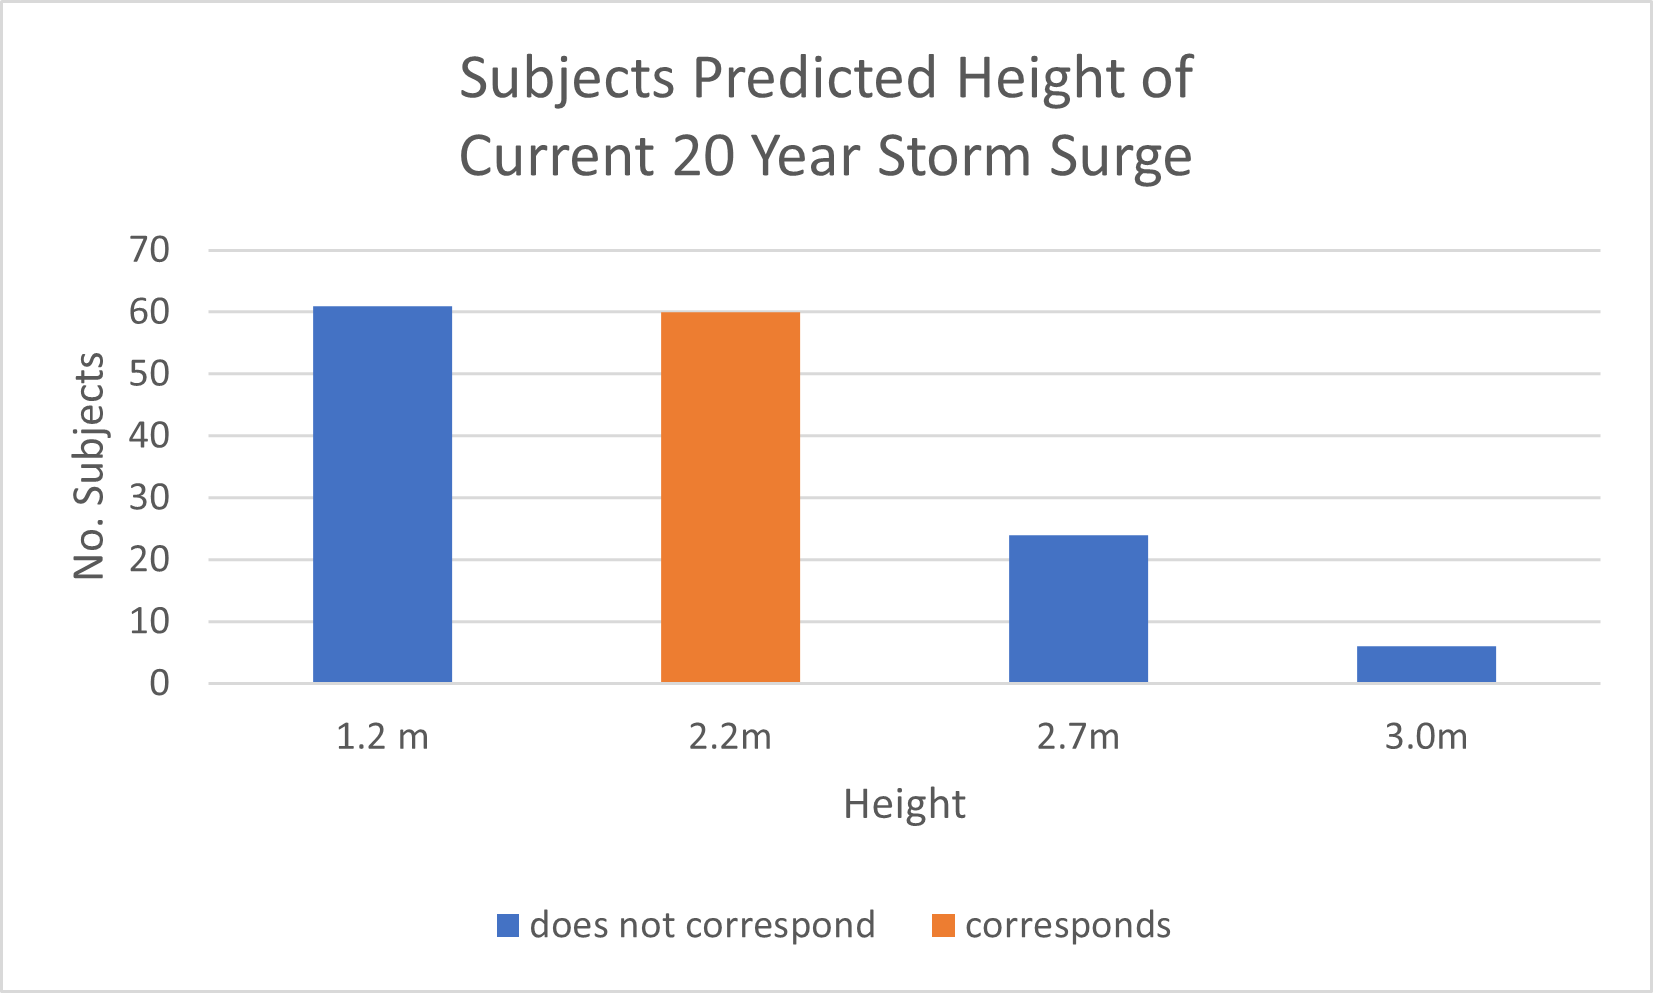
\includegraphics{fig_results/2022-20yrss-answer.png}
    \caption{Subjects Predicted Height of Current 20 Year Storm Surge. 61 subjects chose 1.2m this is very comparable to the 60 which chose 2.2m which is the answer which corresponds with \cite{kartverket_se_2021}. 24 subjects chose 2.7m and only 6 subjectts chose 3.0m}
    \label{fig:2022-stormsurge-answers}
\end{figure}
\paragraph{}
The majority of subjects chose 1.2m as the predicted height of the 20 year storm surge, this does not correspond with models from \cite{kartverket_se_2021}. In fact 1.2m is equal to the current high tide. Almost equally well chosen was the answer which does correspond with models from \cite{kartverket_se_2021}, 2.2m, with 60 subjects choosing this answer. This means that 43 percent of subjects chose the answer which corresponds with \cite{kartverket_se_2021}.

\begin{figure}[h]
    \centering
    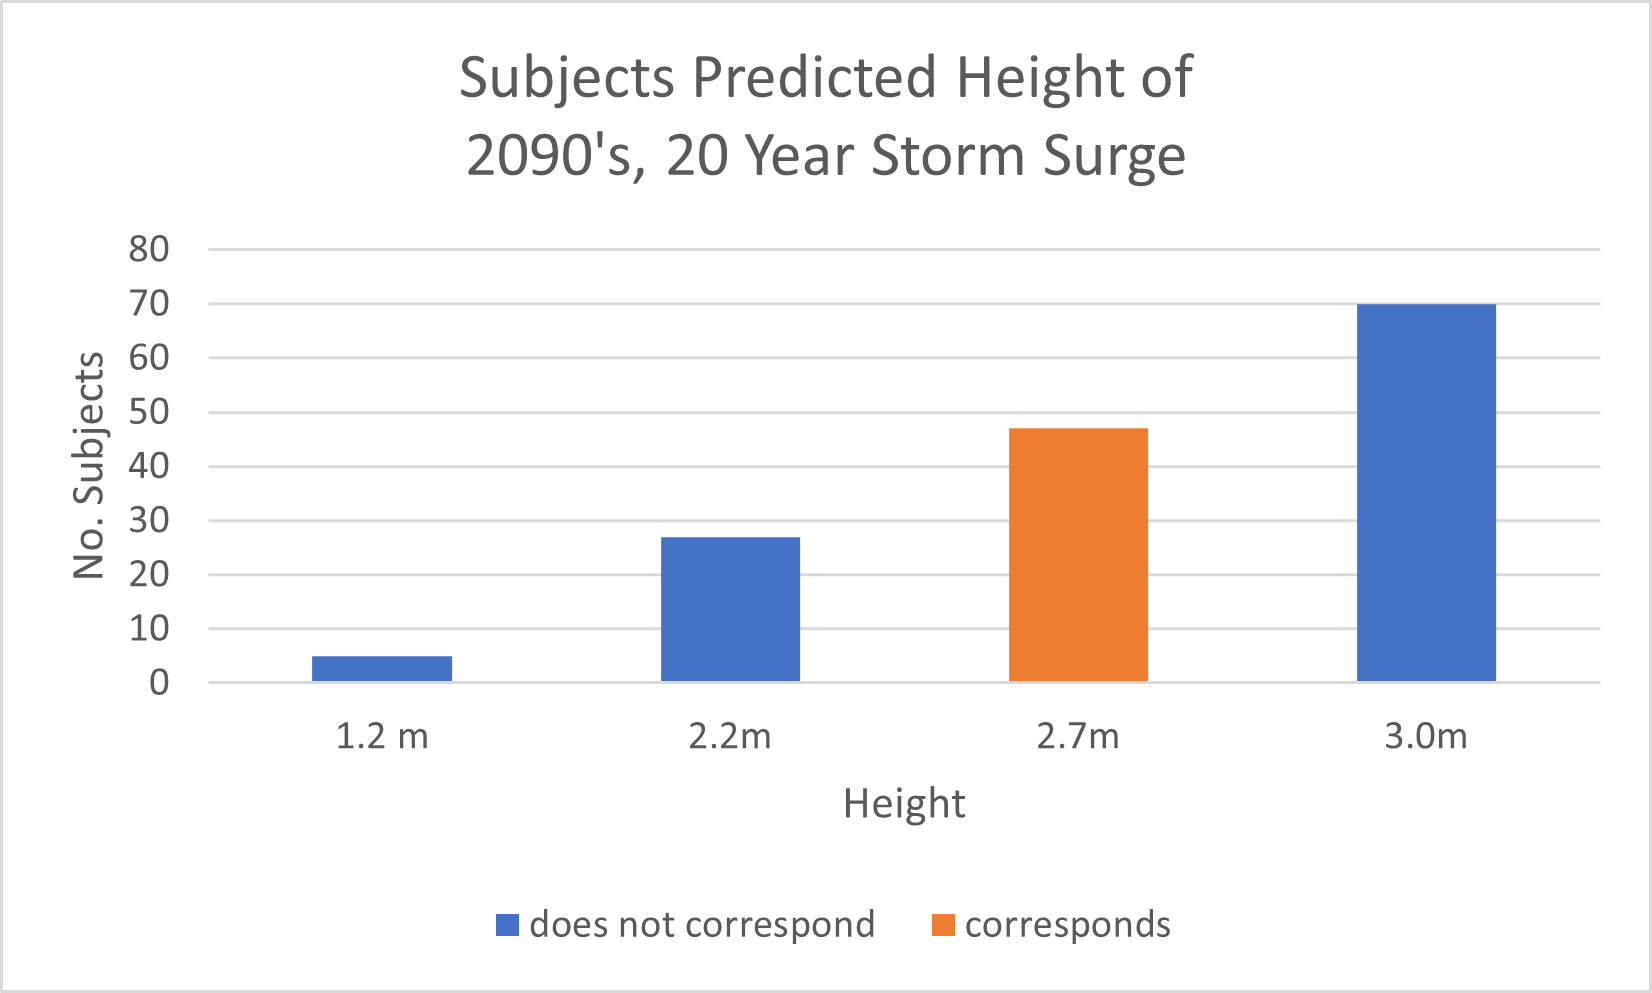
\includegraphics{fig_results/2090s 20yr ss answers.png}
    \caption{Subjects Predicted Height of 2090's, 20 year storm surge. The majority of subjects chose the highest value with 70 subjects choosing 3.0m as the predicted height of the storm surge. 47 subjects chose 2.7m which is the value which corresponds with models by \cite{kartverket_se_2021}. 27 subjects chose 2.2m and only 5 subjects chose 1.2m}
    \label{fig:2090-stormsurge-answers}
\end{figure}
\paragraph{}
The majority of subjects predicted the storm surge in 2090 to be 3.0m. Just over 30 percent chose 2.7m which is the value which corresponds with models from \cite{kartverket_se_2021}. This means that most people thought the sea level extreme associated with the 20 year storm surge in 2090 is higher than it is currently predicted to be. The change of height for the 20 year storm surge predicted for 2090 is only 50cm higher than the current 20 year storm surge \cite{kartverket_se_2021}. 
\paragraph{}

\begin{figure}
    \centering
    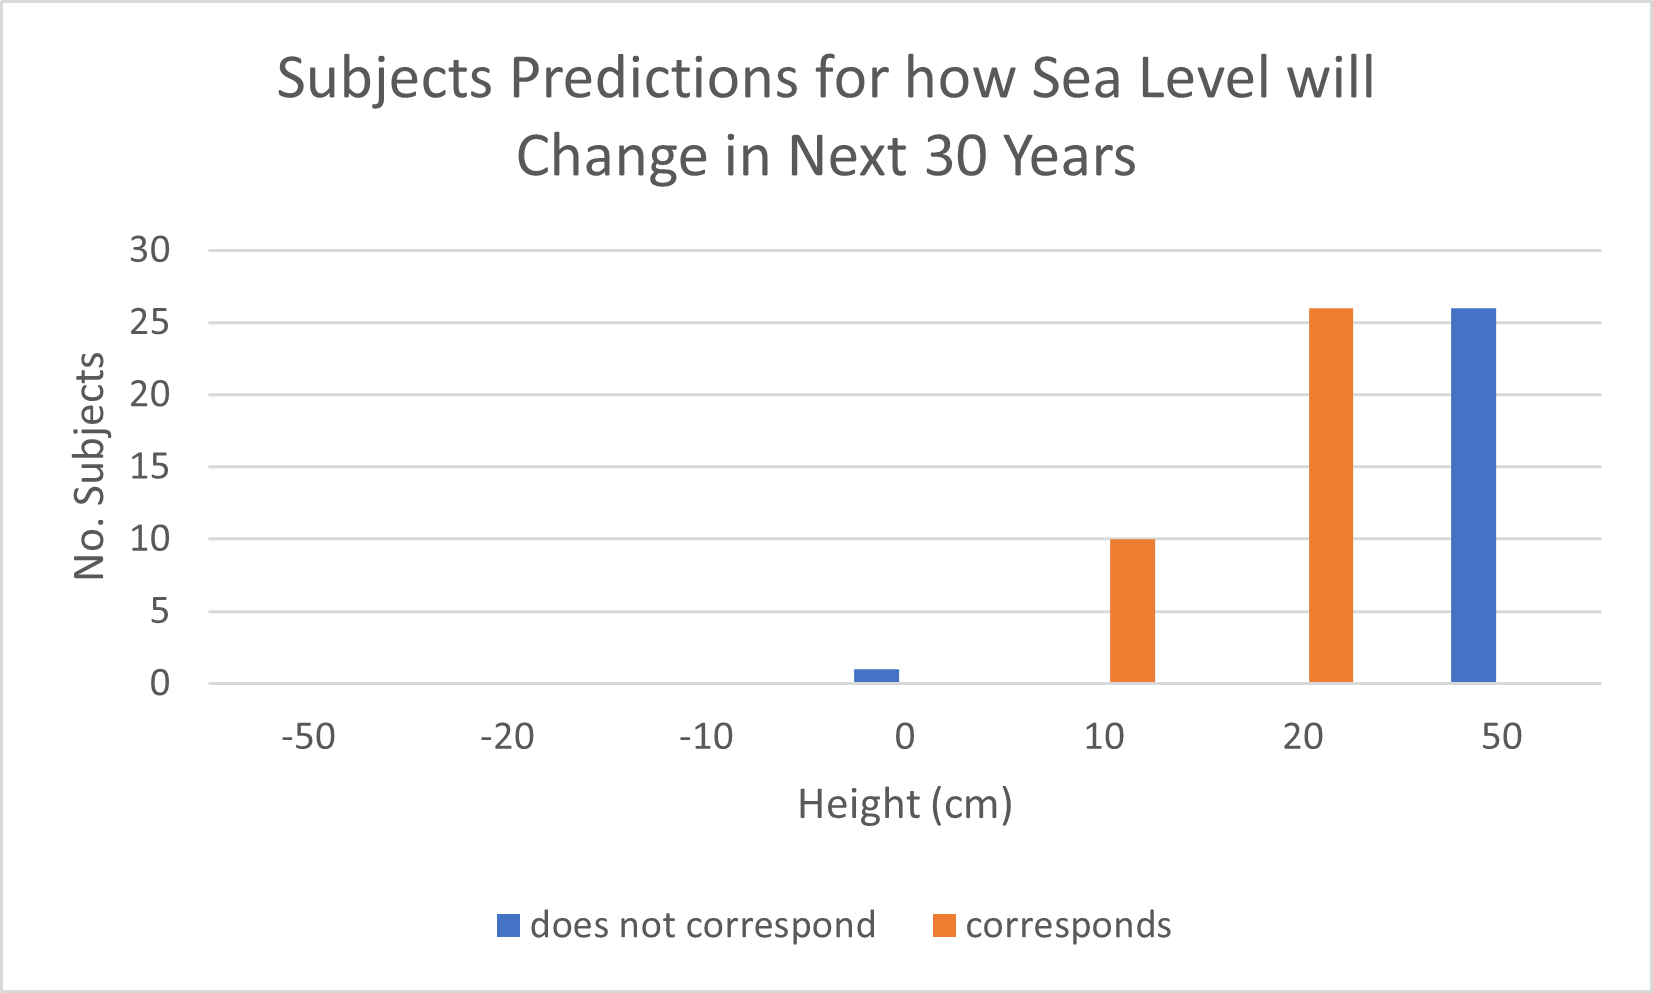
\includegraphics{fig_results/slr-future.png}
    \caption{Subjects Predictions for how Sea Level will change in Trondheim in Next 30 years. Only 147 subjects answered for this question, unlike every other one which all subjects, 153, answered. No subjects believed the sea level will decrease over the next 30 years. One subject answered that it will stay the same, with every other subject chosing that it will rise by some level }
    \label{fig:my_label}
\end{figure}

There is strong uncertainty with this measurement in models, due to the unknown of emisson patterns over the next 30 years and isostatic uplift. Never the less an estimation of 20cm or 10cm is in line with \cite{kartverket_se_2021} which uses the upper emissions pathways from the IPCC. Over half of subjects chose an answer which is in line with models from \cite{kartverket_se_2021}. However equal numbers of subjects,26, chose 50cm which is not in line with these models as chose 20cm. Almost all subjects answered that sea level will rise in the next 30 years, though six subjects chose not to answer this question.  

\begin{figure}
    \centering
    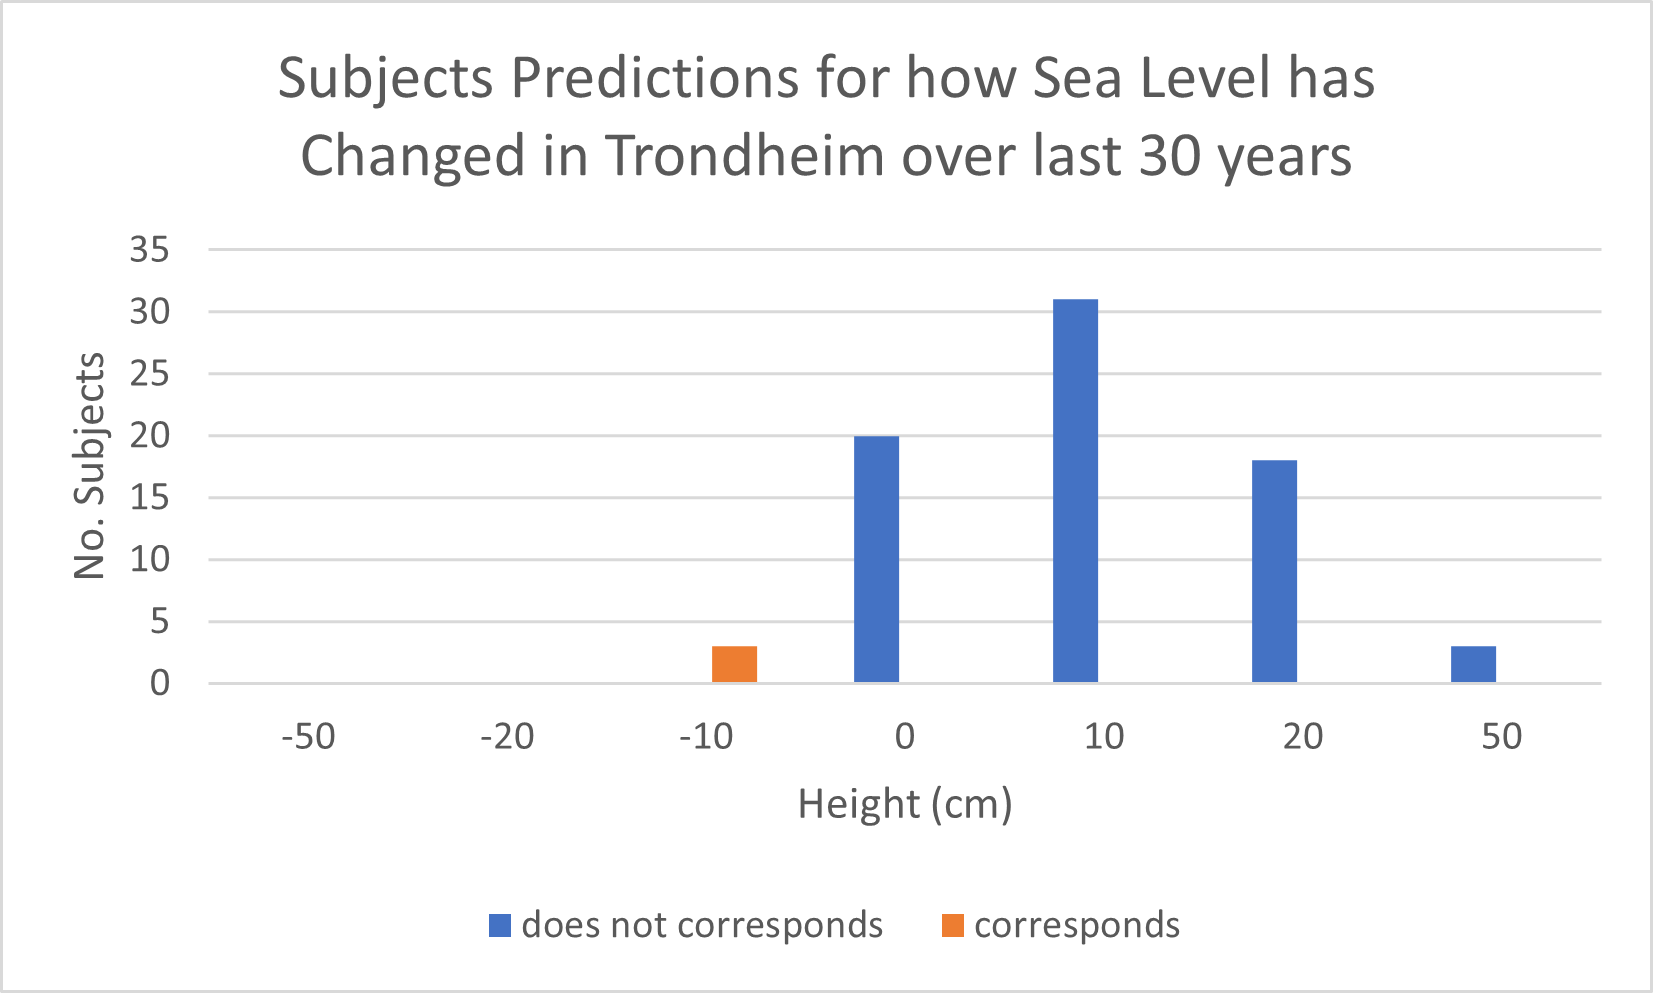
\includegraphics{fig_results/slr-past.png}
    \caption{Subjects Predictions for how Sea Level has Changed in Trondheim over last 30 years. Only 3 subjects chose that sea level has decreased in the last 30 years, this answer is inline with \cite{kartverket_se_2021}. 20 subjects answered that sea level had not changed over this time. While 31 subjects answered that it had risen by 10 cm. 18 subjects answered that it had risen by 20 cm and 3 answered that it had risen by 50 cm. 52 subjects answered that sea level had risen over the last 30 years. }
    \label{fig:my_label}
\end{figure}

The next figure also 
\begin{figure}
    \centering
    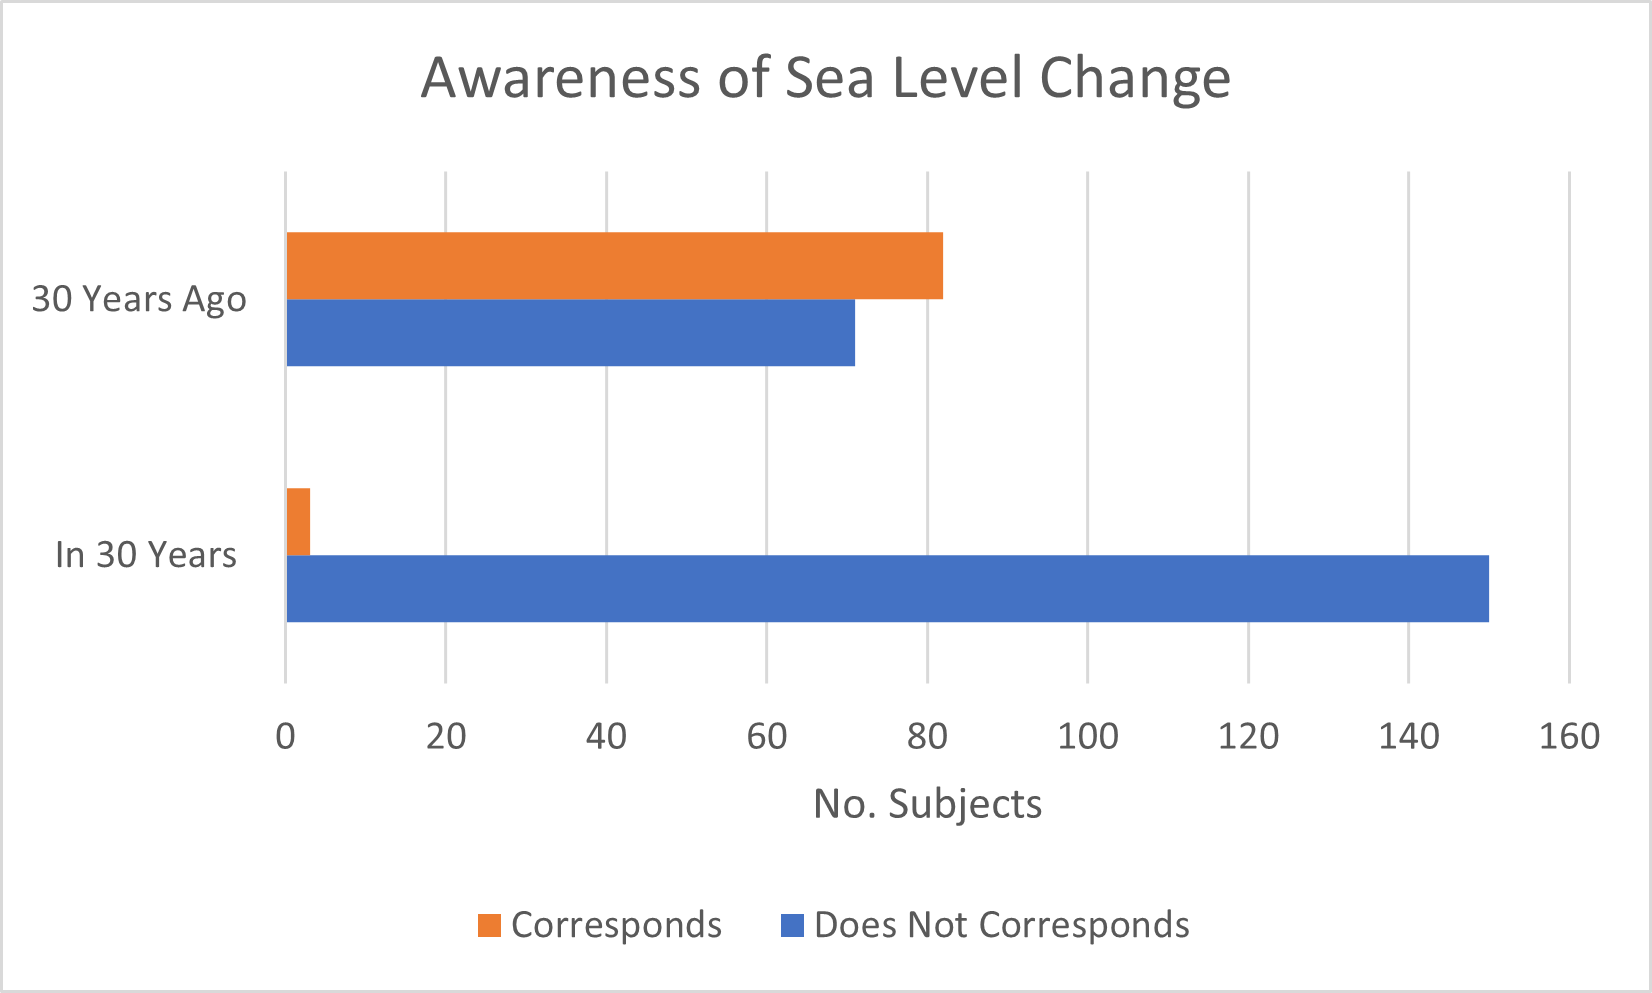
\includegraphics{fig_results/Aware_sea_level_change.png}
    \caption{Awareness of Sea Level Change. Only 3 subjects chose an answer which correpsponds with the models from \cite{kartverket_se_2021}, for what height sea level in Trondheim will be in 20 years time. In contrast 82 subjects just over half chose an answer which corresponds with models from \cite{kartverket_se_2021} for what the sea level was 30 years ago. }
    \label{fig:my_label}
\end{figure}
\paragraph{}

For both of these questions 

Figure.... below is the sum of all results pictured above in this section on awareness. This was the first attempt to determine awareness of subjects from the results of this survey

\begin{figure}
    \centering
    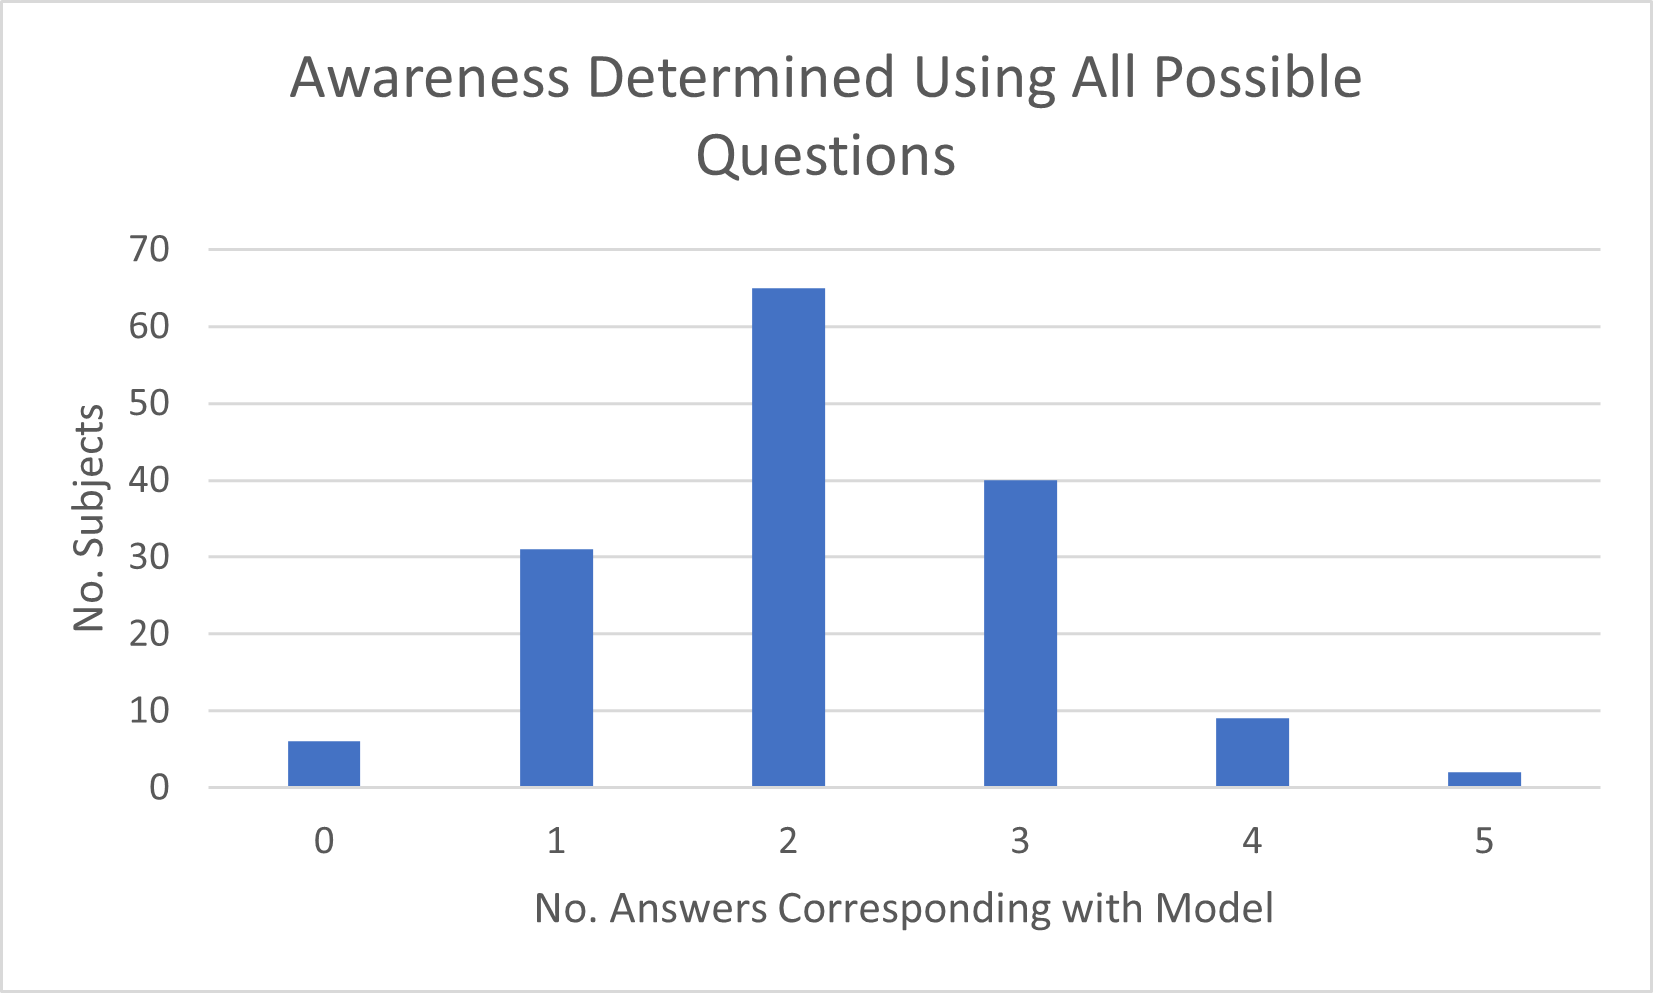
\includegraphics{fig_results/aware_all.png}
    \caption{Caption}
    \label{fig:my_label}
\end{figure}
\paragraph{}

Not very aware - want better split - new determination of awareness -> excluse awareness of sea level change from it 

\begin{figure}
    \centering
    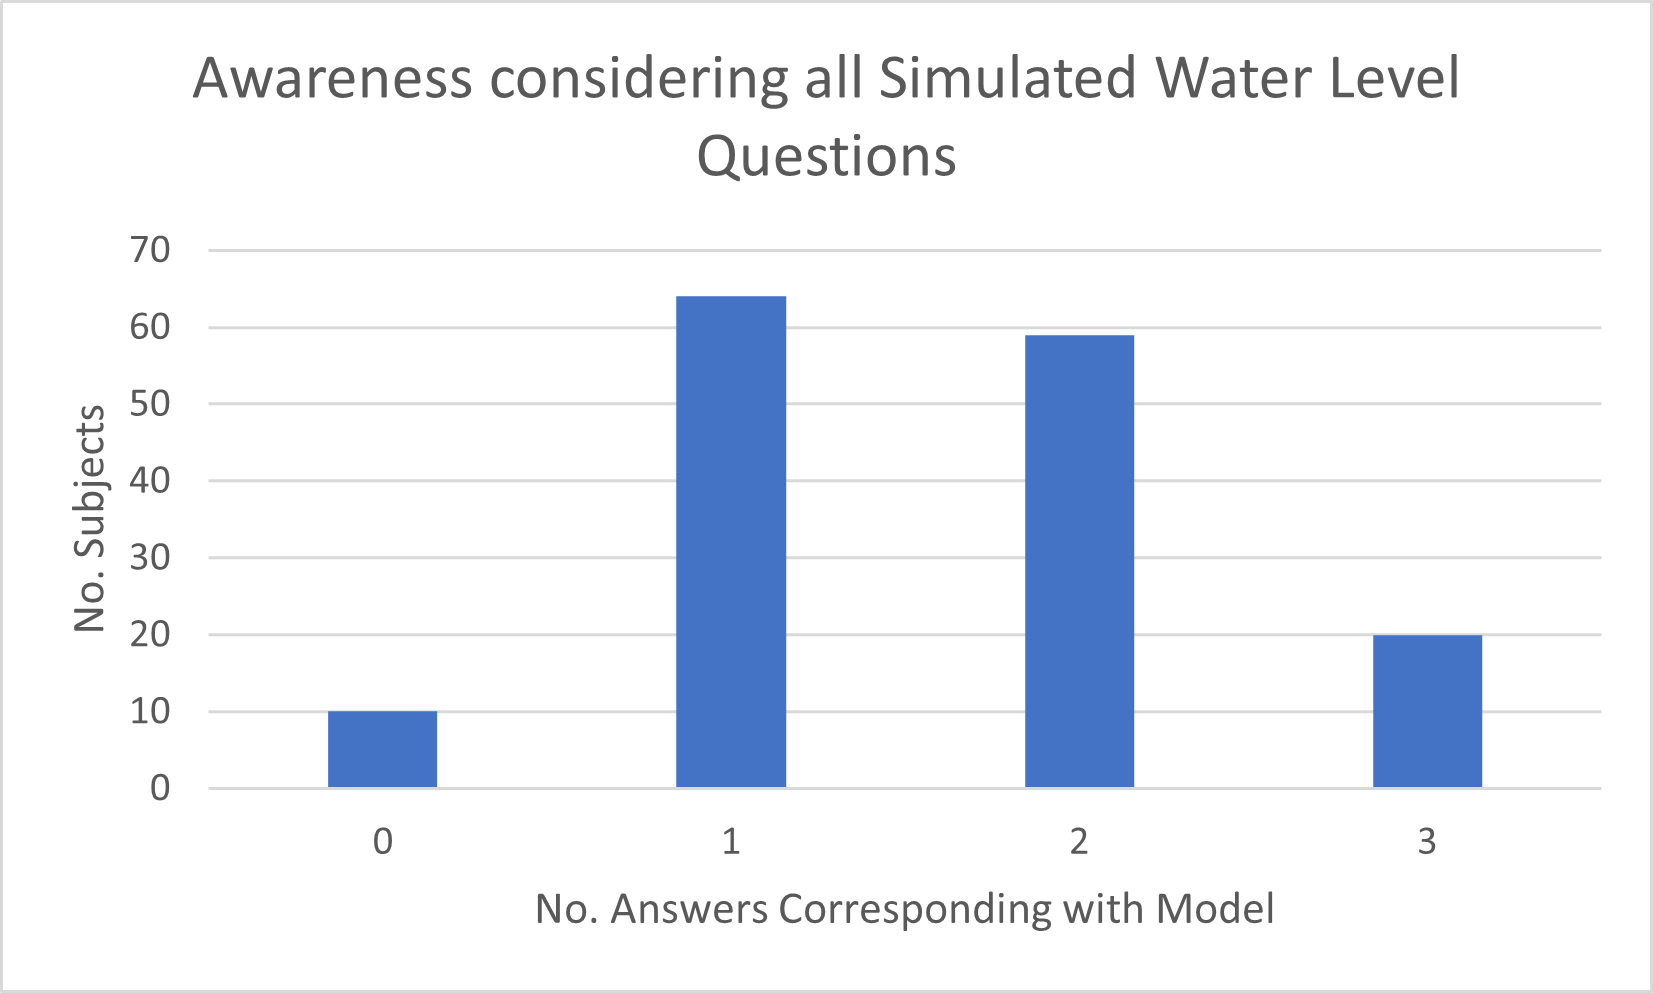
\includegraphics{fig_results/Awareness_ all_simulation_pictures_qs.png}
    \caption{Caption}
    \label{fig:my_label}
\end{figure}